	\documentclass[10pt,oneside]{CBFT_book}
	
	% Algunos paquetes
	\usepackage{amsmath}
	\usepackage{amssymb}
	\usepackage{graphicx}
	\usepackage{libertine}
	\usepackage{lipsum}
	\usepackage[numbers]{natbib}
	\setcitestyle{square}


	\usepackage{polyglossia}
	\setdefaultlanguage{spanish}

	\usepackage{CBFT.estilo} % Cargo la hoja de estilo
	

	% Tipografías
	% \setromanfont[Mapping=tex-text]{Linux Libertine O}
	% \setsansfont[Mapping=tex-text]{DejaVu Sans}
	% \setmonofont[Mapping=tex-text]{DejaVu Sans Mono}

	%===================================================================
	%	DOCUMENTO PROPIAMENTE DICHO
	%===================================================================

% \title{CBFT Mecánica clásica}
% \author{Mecánica lagrangiana}
% \date{\today}

\begin{document}
% \maketitle
% \tableofcontents
\chapter{Conceptos de mecánica newtoniana}

Tal vez sea una simplificación, pero no una muy terrible, decir que el curso de mecánica clásica
busca reemplazar la mecánica basada en las ecuaciones de Newton,
\[
	\vb{F} = m \vb{a} 
\]
por un \emph{formalismo} más poderoso y que se podrá aplicar luego a otros campos.
Este formalismo constituye el corazón de la mecánica clásica.

El contenido de este capítulo forma un núcleo básico de los resultados de le mecánica newtoniana que necesitaremos 
tener a mano para lo subsiguiente (leyes de conservación del momento lineal, momento angular y energía) así como 
ciertos rudimentos mínimos de la matemática usual en la resolución de los problemas.

% =================================================================================================
\section{Leyes de conservación}
% =================================================================================================

Repasaremos a continuación las leyes de conservación fundamentales de la mecánica para sistemas de partículas.

\subsection{Momento lineal}

La segunda ley de Newton se podía escribir en función del momento lineal de una partícula de masa $ m $ como
\[
	\dtot{\vb{p}}{t} = \vb{F}
\]
siendo $ \vb{p} = m\vb{v} $ el momento de la partícula y $ \vb{F} $ la fuerza total que actuaba sobre la misma.
Si el resultado de las fuerzas sobre la partícula era nulo entonces se tiene que $ \vb{p} = cte. $ (el momento lineal 
es una constante de movimiento).

En el caso de un sistema de $N$ partículas como el mostrado en la Figura \ref{fig_mc_leyes_cons} el momento total del 
sistema es la suma de los momentos individuales, es decir
\[
	\vb{P} = \Sum{i=1}{N} \vb{p}_i = \Sum{i=1}{N} m_i \vb{v}_i = \Sum{i=1}{N} m_i \dtot{\vb{x}_i}{t}
\]
luego la segunda ley para el sistema serán las $ N $ ecuaciones
\[
	\dtot{\vb{P}}{t} = \Sum{i=1}{N} m_i \dtot[2]{\vb{x}_i}{t} = \Sum{i=1}{N} \vb{F}_i
\]
donde $ \vb{F}_i$ es la fuerza total sobre la partícula $i$-ésima que puede descomponerse según
\be
	\vb{F}_i = \vb{F}_i^\text{ext} + \Sum{ j \neq i }{N} \vb{F}_{ij}
	\label{descomp_fuerzas}
\ee
siendo $ \vb{F}_i^\text{ext} $ las fuerzas debidas a agentes externos y $\vb{F}_{ij}$ la fuerza sobre la partícula $i$ 
debido a la partícula $j$.

\begin{figure}[hbt]
	\begin{center}
	\includegraphics[width=0.6\textwidth]{images/fig_mc_leyes_cons.pdf}
	\end{center}
	\caption{Sistema de partículas de masas $m_i$ con sus correspondientes vectores de
	posición $\vb{x}_i$. La partícula $m_1$ tiene además indicado su vector velocidad $\vb{v}_1$.}
	\label{fig_mc_leyes_cons}
\end{figure} 

Entonces 
\[
	\dtot{\vb{P}}{t} = \Sum{i=1}{N} m_i \dtot[2]{\vb{x}_i}{t} = \Sum{i=1}{N} \vb{F}_i^\text{ext} + 
	\Sum{i=1}{N} \Sum{ j \neq i }{N} \vb{F}_{ij}
\]
pero el último término del RHS es nulo puesto que por cada sumando $ \vb{F}_{ij} $ también aparece el sumando 
$ \vb{F}_{ji} $ y por acción y reacción estas fuerzas tienen la misma dirección y sentido opuesto, i.e.
\[
	\vb{F}_{ij} = - \vb{F}_{ji}.
\]

De esta forma la ley de conservación para el sistema es 
\[
	\dtot{\vb{P}}{t} = \Sum{i=1}{N} \vb{F}_i^\text{ext} = \vb{F}^\text{ext}_\text{total}
\]
y el momento $ \vb{P} $ del sistema se conserva si la resultante de todas las fuerzas externas es nula. 

Definiendo el vector de posición del centro de masa como 
\[
	\vb{x}_\text{cm} = \frac{\sum_i m_i \vb{x}_i }{\sum_i m_i} = \frac{\sum_i m_i \vb{x}_i }{M}
\]
donde $ M $ es la masa del sistema, se tiene el resultado clásico de que
\[
	\dtot{}{t}( M \vb{x}_\text{cm} ) = \Sum{i=1}{N} m_i \vb{v}_i = M \vb{v}_\text{cm} = \vb{P},
\]
el sistema como un todo tiene un momento total que puede asociársele al de una única partícula {\it centro de masa} de 
masa $M$ y que se mueve con velocidad $ \vb{v}_\text{cm} $.

Si $\vb{P}$ se conserva, entonces $ \vb{v}_\text{cm} $ es una constante, el sistema posee un punto (el centro de masas) 
que se mueve con velocidad constante sin importar qué tan complejo sea el movimiento del conjunto total.

% ~~~~~~~~~~~~~~~~~~~~~~~~~~~~~~~~~~~~~~~~~~~~~~~~~~~~~~~~~~~~~~~~~~~~~~~~~~~~~~~~~~~~~~~~~~~~~~~~~~~~~~~~~~~~~~~~~~~~~
\subsection{Momento angular}

El momento angular de una partícula con momento lineal \vb{p} es 
\[
	\vb{l} = \vb{x} \times \vb{p} = m \: \vb{x} \times \vb{v}.
\]
% El hecho de entre el vector de posición de la partícula en su definición implica que el momento angular
% dependerá del origen del sistema de coordenadas elegido y por ende también su conservación. 
En la Figura 
\ref{fig_mc_mom_ang_particula} se ilustra sobre la trayectoria de una partícula el vector momento angular. 
La variación temporal del momento angular,
\[
	\dtot{\vb{l}}{t} = \dtot{\vb{x}}{t} \times \vb{p} + \vb{x} \times \dtot{\vb{p}}{t} 
\]
se reduce al segundo término, puesto que $ d\vb{x}/dt = \vb{v} $ es paralela a $ \vb{p} $, y
se tiene finalmente el resultado conocido
\be
	\dtot{\vb{l}}{t} = \vb{x} \times \dtot{\vb{p}}{t} = \vb{x} \times \vb{F} = \vb{\tau}
	\label{conserv_mom_ang}
\ee
de que la variación del momento angular es el torque $\vb{\tau}$ causado por la fuerza $ \vb{F} $ 
que actúa sobre la partícula.

\notamargen{Cambiar en el dibujo f por F. Igualmente habría que ser consistente con qué quiero decir
para las mayúsculas y qué para las minúsculas.}
\begin{figure}[hbt]
	\begin{center}
	\includegraphics[width=0.6\textwidth]{images/fig_mc_mom_ang_particula.pdf}	
	\end{center}
	\caption{Una partícula de masa $m$ se desplaza en una trayectoria. En un punto \vb{x} de la misma se
	indican su velocidad \vb{v}, su momento angular \vb{l} y la fuerza \vb{F} a la que está sometida y el
	torque resultante \vb{\tau} por esa fuerza.
	El momento angular es perpendicular al plano (en marrón) definido por los vectores \vb{x} y \vb{v} mientras que 
	el torque lo es al plano (en gris) definido por \vb{x} y \vb{F}.}
	\label{fig_mc_mom_ang_particula}
\end{figure} 

Dado que la definición de $ \vb{l} $ y de $ \vb{\tau} $ implica el vector de posición $ \vb{x} $ se sigue que ambas 
magnitudes dependen de la elección del origen del sistema de coordenadas. 
Es decir que una determinación de $ \vb{l} $ y $ \vb{\tau} $ tiene sentido únicamente con respecto a un cierto origen 
de coordenadas.

De la ecuación \eqref{conserv_mom_ang} se deduce que si la fuerza es siempre paralela al vector de posición de una 
partícula ($\vb{F} \parallel \vb{x}$) entonces el momento angular \vb{l} se conserva puesto que el torque es 
$\vb{\tau}=0$ en ese caso. Es lo que se llama una fuerza central.
\notamargen{Habría que destacar lo de fuerza central con un dibujo. Es importante.}

\subsubsection{Momento angular para un sistema de partículas}

Si ahora tenemos un sistema de $N$ partículas el momento angular correspondiente (con respecto a un dado origen de
coordenadas) será
\[
	\vb{L} = \Sum{i=1}{N} \: \vb{x}_i \times \vb{p}_i
\]

De manera equivalente, la variación temporal es 
\[
	\dtot{\vb{L}}{t} = \Sum{i=1}{N} \vb{x}_i \times \vb{F}_i
\]
y si utilizamos la descomposición \eqref{descomp_fuerzas} para la fuerza $\vb{F}_i$ resulta
\[
	\dtot{\vb{L}}{t} = \Sum{i=1}{N} \vb{x}_i \times \vb{F}_i^\text{ext}  +
	\Sum{i=1}{N} \Sum{j\neq i}{N}  \vb{x}_i \times \vb{F}_{ij}
\]

Es claro\footnote{Nota \ref{nota_suma_ineqj}} que el segundo término puede expresarse de manera equivalente como 
\[
	\Sum{i=1}{N} \Sum{j\neq i}{N}  \vb{x}_i \times \vb{F}_{ij} =
	\frac{1}{2} 
	\Sum{i=1}{N} \Sum{j \neq i}{N}  \left[ \vb{x}_i \times \vb{F}_{ij} + \vb{x}_j \times \vb{F}_{ji} \right]
\]
y aceptando que las fuerzas internas son pares acción-reacción se tiene 
\[
	\Sum{i=1}{N} \Sum{j\neq i}{N}  \vb{x}_i \times \vb{F}_{ij} =
	\frac{1}{2} 
	\Sum{i=1}{N} \Sum{j \neq i}{N}  \left[ \vb{x}_i - \vb{x}_j \right] \times \vb{F}_{ij},
\]
de manera que la derivada del momento angular total es 
\be
	\dtot{\vb{L}}{t} = \Sum{i=1}{N} \vb{x}_i \times \vb{F}_i^\text{ext}  +
	\frac{1}{2} \Sum{i=1}{N} \Sum{j \neq i}{N}  \left[ \vb{x}_i - \vb{x}_j \right] \times \vb{F}_{ij} 
	\label{dL_sistema}
\ee

La conservación de \vb{L},
\[
	\dtot{\vb{L}}{t} = 0	
\]
requiere entonces que las fuerzas externas sean centrales, lo cual anula el primer término en \eqref{dL_sistema},
y que se verifique 
\[
	\vb{F}_{ij}  \parallel ( \vb{x}_i - \vb{x}_j ),
\]
es decir que la fuerza sobre $i$ ejercida por la partícula $j$ tenga la dirección del vector que une las dos 
partículas, para anular el segundo término de \eqref{dL_sistema}.

\begin{figure}[htb]
	\begin{center}
	\includegraphics[width=0.4\textwidth]{images/fig_mc_parstrong.pdf}	
	\end{center}
	\caption{Principio de acción y reacción fuerte para dos partículas de masas $m_i$ y $m_j$.}
	\label{fig_mc_parstrong}
\end{figure} 

Esto establece lo que se llama un ``principio de acción y reacción {\it fuerte}''; las fuerzas son iguales y opuestas 
(de esto se trata el principio de acción y reacción), pero además colineales.
Dadas dos partículas del sistema cualesquiera con posiciones $ \vb{x}_i, \vb{x}_j $ y de masas $ m_i, m_j $, como se 
muestra en la Figura \ref{fig_mc_parstrong}, la fuerza $\vb{F}_{ij}$ sobre $i$ debido a $j$ debe estar contenida en la 
dirección del vector $ \vb{x}_i - \vb{x}_j $ lo cual le otorga las dos posibilidades indicadas por las flechas rojas 
gruesas. Para la fuerza $\vb{F}_{ji}$ el razonamiento es, por supuesto, idéntico.

\notamargen{Acá hay más para extraer: poner un gráfico con lo que no puede pasar. Poner un código de colores para
las flechas, puesto que si son iguales y opuestas las fuerzas están hermanadas las externas por un lado y las internas
por el otro.}

La existencia de un principio de acción y reacción fuerte sobreviene [es una consecuencia?] de la naturaleza puntual de 
los cuerpos. De no ser puntuales se tendrá principio de acción y reacción a secas.

Existe otra descomposición interesante para el momento angular \vb{L} de un sistema de $N$ partículas en términos de 
sus distancias al centro de masas.

Para cada partícula $i$-ésima con posición $ \vb{x}_i $ y velocidad $ \vb{v}_i $ definimos una coordenada $ \vb{x}_i' $ 
y una velocidad $\vb{v}_i' $ en términos de la posición \vb{X} y velocidad \vb{V} del centro de masa, ver Figura 
\ref{fig_mc_angularmom}, de acuerdo a
\[
	\vb{x}_i = \vb{X} + \vb{x}_i' \qquad \vb{v}_i = \vb{V} + \vb{v}_i',
\]
es decir que consideramos coordenadas respecto al centro de masa.

\begin{figure}[hbt]
	\begin{center}
	\includegraphics[width=0.6\textwidth]{images/fig_mc_angularmom.pdf}	
	\end{center}
	\caption{}
	\label{fig_mc_angularmom}
\end{figure} 

\notamargen{Actualizar el $X_{cm}$ en el gráfico y poner el origen O.}

En términos de estas nuevas variables primadas el momento angular es
\[
	\vb{L}_O = \Sum{i=1}{N} \vb{x}_i \times \vb{p}_i = 
	\Sum{i=1}{N} (\vb{X} + \vb{x}_i') \times m_i (\vb{V} + \vb{v}_i')
\]
\[
	\vb{L}_O = \Sum{i=1}{N} ( \vb{X} \times m_i \vb{V}  + \vb{X} \times m_i \vb{v}_i'
	+ \vb{x}_i' \times m_i \vb{V} 	+ \vb{x}_i' \times m_i \vb{v}_i' )
\]

Como la posición del centro de masa es
\be
	\vb{X} = \frac{1}{M} \Sum{i=1}{N} m_i \vb{x}_i  
	\label{R_cm}
\ee
se tendrá 
\[
	M \vb{X} = \Sum{i=1}{N} m_i \vb{x}_i = \Sum{i=1}{N} m_i ( \vb{X} + \vb{x}_i' ) =
	\vb{X} \Sum{i=1}{N} m_i + \Sum{i=1}{N} m_i \vb{x}_i'
\]
pero el primer término del RHS es $M\vb{X}$ de manera que 
\be
	\Sum{i=1}{N} m_i \vb{x}_i' = 0 .
	\label{Condicion_cm}
\ee
La velocidad del centro de masa es la derivada temporal de \eqref{R_cm}, i.e.
\be
	\vb{V} = \frac{1}{M} \Sum{i=1}{N} m_i \dtot{\vb{x}_i}{t} = 
	\frac{1}{M} \Sum{i=1}{N} m_i \vb{v}_i
	\label{V_cm}
\ee

Con estos resultados volvemos a la expresión del momento que resulta 
\[
	\vb{L}_O = \vb{X} \times M \vb{V}  + \vb{X} \times \left( \Sum{i=1}{N} m_i \vb{v}_i' \right) +
	\left( \Sum{i=1}{N} m_i \vb{x}_i' \right) \times \vb{V} + \Sum{i=1}{N} \vb{x}_i' \times m_i \vb{v}_i',
\]
pero debido a \eqref{Condicion_cm} y a su derivada temporal (que resulta nula) el segundo y tercer sumando de la 
expresión anterior son nulos y entonces 
\[
	\vb{L}_O = \left( \vb{X} \times M \vb{V} \right) + \Sum{i=1}{N} ( \vb{x}_i' \times m_i \vb{v}_i' )
\]
% \[
% 	\vb{L}^T_O = \vb{L}^{cm} + \vb{L}^{sist}_{cm}
% \]
siendo el primer término del RHS el momento angular orbital y el segundo el momento angular de spin.

% Con respecto a la conservacion del momento angular, se tendrá
% \[
% 	\dtot{\vb{L}_O}{t} = \sum \vb{\tau}_O
% \]
% que se puede ver como suma del torque de fuerzas externas y de fuerzas internas. En el primer caso,
% los torques externos sumarán cero si las fuerzas externas son nulas o centrales.
% En el segundo caso los torques internos son nulos si vale el principio de acción y reacción fuerte;
% es decir si
% \[
% 	\vb{r}_i - \vb{r}_j \parallel F_{ij}.
% \]

% ~~~~~~~~~~~~~~~~~~~~~~~~~~~~~~~~~~~~~~~~~~~~~~~~~~~~~~~~~~~~~~~~~~~~~~~~~~~~~~~~~~~~~~~~~~~~~~~~~~~~~~~~~~~~~~~~~~~~~
\subsection{Trabajo y energía}

Consideremos una partícula de masa $ m $ que se mueve sobre una cierta trayectoria suave $\vb{x}(t)$, ver {Figura} 
\ref{fig_mc_workenergy}, debido a la acción de una fuerza \vb{F}.
Su velocidad \vb{v} es en todo momento tangente a la trayectoria y define de esta forma un versor $ \hat{t} $
colineal con la misma. Esto define un plano, mostrado en la parte derecha de la figura, para el cual todo vector
perteneciente al mismo es normal a la trayectoria. Elegimos un versor $ \hat{n} $ que está en la dirección de
la proyección de \vb{F} sobre dicho plano.

\begin{figure}[!h]
	\begin{center}
	\includegraphics[width=0.9\textwidth]{images/fig_mc_workandenergy.pdf}	
	\end{center}
	\caption{Partícula de masa $m$ que se mueve sobre una trayectoria $\vb{x}(t)$ bajo la acción de una fuerza 
\vb{F} (izquierda). En el detalle de la derecha se muestra la descomposición del movimiento en direcciones
tangencial $\hat{t}$ y normal $\hat{n}$.}
	\label{fig_mc_workenergy}
\end{figure} 

Descomponiendo la fuerza y la velocidad en estas dos direcciones, se tiene 
\[
	\vb{F} = F^t \: \hat{t}  + F^n \: \hat{n} \qquad \qquad \vb{v} = v \: \hat{t}
\]
de manera que la segunda ley de Newton, 
\[
	m \: \dtot{\vb{v}}{t} = \vb{F},
\]
para la componente $\hat{t}$ resulta
\[
	m \dtot{v}{t} = F^t
\]
\notamargen{Notemos que el versor desplazamiento $d\vb{s}$ {\it camina} por la trayectoria.}
Involucrando al diferencial de arco $ ds = | d\vb{x} | $ a lo largo de la trayectoria, la ecuación anterior se
puede escribir como
\be
	m \: dv \:\dtot{s}{t} = m \: v \: dv = F^t \: ds = \vb{F} \cdot d\vb{x},
	\label{ec_trabajo}
\ee
donde la última igualdad es posible en virtud de que $ F^n \perp d\vb{x} $ por construcción.

Podemos integrar ambos miembros de \eqref{ec_trabajo} entre $\vb{x}(t_0) \equiv \vb{x}_0$ y su 
correspondiente velocidad $v(t_0) \equiv v_0$ hasta $\vb{x}_1, \vb{v}_1$, 
\[
	m \int_{v_0}^{v_1} \: v \: dv = \int_{\vb{x}_0}^{\vb{x}_1}  \vb{F} \cdot d\vb{x}
\]
obteniendo
\[
	\left. \frac{1}{2} m v^2 \right|_{v_0}^{v_1} = W_{\vb{x}_0 \to \vb{x}_1} 
\]
que es el llamado \emph{teorema de las fuerzas vivas} para una partícula de masa $m$ y nos dice que la
variación de energía cinética en la trayectoria es igual al trabajo de todas las fuerzas que actúan
sobre la misma, i.e.
\be
	T_1 - T_0 = \Delta T_{\vb{x}_0 \to \vb{x}_1}  = W_{\vb{x}_0 \to \vb{x}_1} .
	\label{conser_energia}
\ee

En el caso particular en que la fuerza sea normal a la trayectoria en todo el intervalo $[t_0,t_1]$ se 
tendrá $\Delta T = 0 $, es decir que se conserva la energía cinética a lo largo de toda la trayectoria.
Sólo las componentes tangenciales de la fuerza producen trabajo y esto es solamente debido a que este proviene
de un producto escalar (una proyección); las componentes normales no hacen trabajo.

\notamargen{ Falta meter lo de \[ 	 m \frac{v^2}{\rho} = F_n \] }

Si la fuerza proviene de un potencial\footnote{El menos delante del gradiente es una convención, como se verá a
continuación.}, se tiene 
\be
	\vb{F} = - \nabla V
	\label{fuerza_prov_potencial}
\ee
y podemos expresar en coordenadas cartesianas esta equivalencia \eqref{fuerza_prov_potencial}
\[
	\vb{F} = -\left( \dpar{V}{x_1}, \dpar{V}{x_2}, \dpar{V}{x_3} \right)
\]
y evaluar la integral del trabajo para obtener
\[
	W = \int_{\vb{x}_0}^{\vb{x}_1}  \vb{F} \cdot d\vb{x} =
	\int_{t_0}^{t_1}  \vb{F}(\vb{x}[t]) \cdot \dotvb{ x } \: dt =
	- \int_{t_0}^{t_1}  \sum_{i=1}^3 \left[ \dpar{V}{x_i} \dtot{x_i}{t} \right] \: dt = V_0 - V_1
\]
donde la última igualdad se obtiene por integración de un gradiente. Esto 
significa que la integral es independiente de la trayectoria $\vb{x}_0 \to \vb{x}_1$.

Entonces, volviendo a \eqref{conser_energia}
\[
 	\rlap{ $\overbrace{\phantom{T_1 - T_0 = W_{0 \to 1}}}^{\text{Vale siempre}} $}  T_1 - T_0 =
	\underbrace{ W_{0 \to 1} = V_0 - V_1 }_{\text{Si $\vb{F}$ proviene de potencial} }
\]
y pasando de miembros se tiene 
\[
	(T_1 + V_1) = (T_0 + V_0 ) 
\]
que viene a significar que la cantidad $ E = T + V $ (la energía mecánica) se conserva si la fuerza $\vb{F}$ 
proviene de un potencial $V$. 
Por dicha razón, las fuerzas para las cuales se verifica \eqref{fuerza_prov_potencial} se llaman {\it fuerzas
conservativas}. En una dimensión, cualquier $ F(x) $ se puede hacer provenir de un potencial si verifica ser
integrable, es decir si podemos definir
\be
	V(x) = \int F(x) \: dx.
	\label{potencial_1d}
\ee
Para tres dimensiones no cualquier $ F(\vb{x}) $ es conservativa.

El signo negativo en \eqref{fuerza_prov_potencial} hace que la cantidad conservada sea $T+V$ en lugar de $T-V$.
Tiene más sentido físico que se conserve una suma de energías antes que una resta de las mismas.

\subsubsection{Trabajo y energía para un sistema de partículas}

Para un sistema de $ N $ partículas la energía cinética simplemente es la suma de las energías cinéticas de cada 
partícula,
\[
	T = \sum_{i=1}^N \: \frac{1}{2} \: m_i v_i^2.
\]

Utilizando la expresión en función del centro de masa, $\vb{v}_i = \vb{V} + \vb{v}_i'$ en la energía se llega a
\[
	T = \frac 1 2 M V^2 + \frac{1}{2} \: \sum_{i=1}^N \: m_i {v_i'}^2,
\]
donde el primer término es la energía cinética de traslación del centro de masa y el segundo término (la sumatoria) es 
la energía cinética interna.
En el caso de dos cuerpos la anterior expresión se reduce a
\[
	T = \frac 1 2 M V^2 + \frac 1 2 \mu v_r^2
\]
donde $\mu$ es la masa reducida y $v_r$ es la velocidad relativa.
\notamargen{Las conservaciones de las cosas permiten reducir la cantidad de integraciones necesarias.}

La definición del trabajo, en cambio, es un poco más complicada. Entre dos instantes de tiempo $ t $ y $ t + \Delta t $ 
el sistema está caracterizado por las $ N $ posiciones $ \{\vb{x}_i\} $ de todos sus integrantes y cada partícula 
experimenta un desplazamiento $ \Delta \vb{x}_i $ asociado con la fuerza que actúa sobre ella.

En principio la fuerza sobre cada partícula puede dividirse en interna (debida a las otras partículas del sistema) y 
externa (debida a agentes exteriores al sistema), lo cual permite escribir
\[
	\vb{F} = \vb{F}^{\text{int}} + \vb{F}^{\text{ext}}
\]
y consecuentemente
\[
	W = W^{\text{int}} + W^{\text{ext}}
\]

El $ W $ entre dos instantes de tiempo $t_0$ y $t_1$ corresponde ahora a la integral entre la configuración del sistema 
a $t_0$ dada por $ \{\vb{x}_i(t_0)\} $ hasta la configuración $ \{\vb{x}_i(t_1)\} $, las cuales etiquetaremos como 0 y 
1 respectivamente. 
\notamargen{El rozamiento depende de la velocidad, entonces no es conservativo.}

Entonces el trabajo externo es
\[
	W^{\text{ext}} = \sum_{i=1}^N \int_0^1 \vb{F}^{\text{ext}}_i \cdot \: d\vb{x}_i
\]
siendo $ \vb{F}^{\text{ext}}_i $ la fuerza externa sobre la partícula $i$. Para que valga la conservatividad es 
necesario que 
\begin{itemize}
 \item La fuerza sobre $i$ dependa solamente de las coordenadas $\vb{x}_i$ de esa partícula. Es decir:
 \[
	\vb{F}_i = \vb{F}_i(\vb{x}_i)
 \]
 \item Se verifique para cada $\vb{F}_i$ 
 \[
	\Nabla \times \vb{F}_i = 0,
 \]
 donde el operador $\nabla$ se toma con respecto a las coordenadas de la partícula $i$ en cuestión.
\end{itemize}

\begin{figure}[!hb]
	\begin{center}
	\includegraphics[width=0.75\textwidth]{images/fig_mc_work_system.pdf}	
	\end{center}
	\caption{Elementos implicados en la evaluación del trabajo interno $ W^{\text{int}} $ para un sistema
	de partículas.}
	\label{fig_mc_work_system}
\end{figure} 

\notamargen{Arreglar flechas en este gráfico.}

Estas condiciones permiten escribir la fuerza como el gradiente de un potencial y entonces el trabajo externo es la 
suma de las diferencias entre las energías potenciales de las partículas entre las configuraciones 0 y 1, o bien
\[
	W^{\text{ext}} = - \sum_{i=1}^N \left. \Delta V_i(\vb{x}_i) \right|_0^1
\]

El trabajo interno corresponde a la suma sobre cada partícula $i$ de la fuerza ejercida por todas las otras partículas 
$j \neq i$ del sistema, es decir
\be
	W^{\text{int}} = \sum_{i=1}^N \sum_{j\neq i}^N \int_0^1 \vb{F}_{ij} \cdot d\vb{x}_i
	\label{internal_work}
\ee
donde $\vb{F}_{ij} $ es la fuerza sobre $i$ ejercida por $j$. La restricción en la sumatoria sobre $j$ descarta la suma 
de autofuerzas. Es claro que la expresión \eqref{internal_work} se puede escribir equivalentemente como
\[
	\frac{1}{2} \sum_{i=1}^N \sum_{j\neq i}^N \int_0^1 
	\left( \vb{F}_{ij} \cdot d\vb{x}_i + \vb{F}_{ji} \cdot d\vb{x}_j \right) 
\]
\notamargen{¿nota final con la justificación de que se puede escribir así?}
% justificación :
% Esta sumatoria tiene N(N-1) términos que resultan de los N por N posibilidades excluyendo los N tales que i=j
% Por cada término del tipo F_ij dx_i hay un correspondiente F_ji dx_j; por ejemplo está F_13 dx_1 (i=1 u j=3) y F_31 
% dx_3 que viene de i=3 y j=1. Luego podemos sumar todo dos veces considerando un sumando general F_ijdx_i + F_jidx_j 
% preo dividiendo por dos para compensar. 
%
y si ahora aceptamos que vale el principio de acción y reacción
\[
	\frac{1}{2} \sum_{i=1}^N \sum_{j\neq i}^N \int_0^1 
	\vb{F}_{ij} \cdot \left(d\vb{x}_i - d\vb{x}_j \right) .
\]
Definiendo luego un vector de separación relativa $ \vb{r}_{ij} = \vb{x}_i - \vb{x}_j $ se tiene que las integrales son 
de la forma 
\[
	\int \vb{F}_{ij} \cdot d\vb{r}_{ij}
\]
y sabemos, por analogía con lo anterior, que si $\vb{F}_{ij}$ depende del vector de separación $ \vb{r}_{ij} $ y es de 
rotor nulo entonces las fuerzas internas son conservativas.
Entonces,
\[
	\vb{F}_{ij} = -\Nabla_i V(\vb{r}_{ij}) \qquad \vb{F}_{ji} = -\Nabla_j V(\vb{r}_{ij})
\]
y como vale acción y reacción $\vb{F}_{ij} = - \vb{F}_{ji}$ esto lleva a que $\nabla_i = \nabla_j$.
\notamargen{Un potencial que depende solo de la distancia entre dos partículas $|r_{ij}|$ cumple PAR fuerte.}

Un ejemplo numérico aclarará esta relación. Sea un potencial que depende de la distancia entre dos partículas,
$r = |\vb{r}_{ij}|$, es decir que si $i=2$ y $j=1$ se tendrá
\[
	r = \sqrt{ (x_2-x_1)^2 + (z_2-z_1)^2 + (z_2-z_1)^2 },
\]
luego,
\begin{multline*}
	\: \vb{F}_{21} = -\Nabla_2 V = -\dpar{V}{r} \left( \dpar{r}{x_2}\hat{x} + \dpar{r}{y_2}\hat{y} + 
	\dpar{r}{z_2}\hat{z} \right) = \\ 
	-\dpar{V}{r} \frac 1 r \left( (x_2-x_1)\hat{x} + (y_2-y_1)\hat{y} + (z_2-z_1)\hat{z} \right)
\end{multline*}
y, en cambio,
\begin{multline*}
	\: \vb{F}_{12} = -\Nabla_1 V = -\dpar{V}{r} \left( \dpar{r}{x_1}\hat{x} + \dpar{r}{y_1}\hat{y} + 
	\dpar{r}{z_1}\hat{z} \right) = \\ 
	-\dpar{V}{r} \frac 1 r \left( -(x_2-x_1)\hat{x} - (y_2-y_1)\hat{y} - (z_2-z_1)\hat{z} \right)
\end{multline*}
de manera que $ \vb{F}_{21} = -\vb{F}_{12} $.

En estos casos, en presencia de fuerzas conservativas
\[
	E = T + V^e(\vb{x}_1,...,\vb{x}_N) + \frac 1 2 \sum_{i=1}^N \sum_{j=1}^N V_{ij}
\]
donde $V^e$ es el trabajo externo. Luego, la variación de energía $\Delta E$ será
\[
	\Delta E = \sum_{i=1}^N ( \Delta T_i - \Delta V_i ) + \frac{1}{2} \sum_{i=1}^N \sum_{j=1}^N \Delta V_{ij}.
\]
\notamargen{Revisar la escritura de la energía y de la variación, qué pienso con respecto a T, V?}


% ~~~~~~~~~~~~~~~~~~~~~~~~~~~~~~~~~~~~~~~~~~~~~~~~~~~~~~~~~~~~~~~~~~~~~~~~~~~~~~~~~~~~~~~~~~~~~~~~~~~~~~~~~~~~~~~~~~~~~
\begin{ejemplo}{\bfseries Análisis energético de un potencial }

\label{ejemplo_analisis_potencial}
Dada una fuerza 1D 
\[
	F(x) = -k x + \frac{a}{x^3} ,	\qquad \qquad a > 0
\]
se realiza un análisis del potencial resultante y de la energía.

\cajacostado{12cm}{12.4cm}{
La fuerza $-kx$ es una fuerza restitutiva mientras que $a/x^3$ es una fuerza
repulsiva pués $a > 0$. 
% También podríamos decir que se tiene:
% \[
% 	\partial \Psi = 0
% \]
}

\vspace*{1mm}
A partir de esta fuerza, que es la del oscilador armónico 1D sumada a una perturbación controlada por el parámetro 
$a$, procedemos a calcular el potencial, a través de la relación \eqref{potencial_1d} de modo que (a menos de una 
constante aditiva que no interesa aquí) se obtiene
\[
	V(x) = \frac{k}{2} x^2 + \frac{a}{2 x^2}
\]
siendo la energía total 
\[
	E = T + V( x ), 
\]
la cual es una cantidad conservada.
% Para analizar el movimiento bajo este potencial consideraremos tres relaciones diferentes entre los parámetros $k,a$ 
% para poder graficar $ V(x) $. Consideraremos tres casos numéricos $ k = 100 a, 20 a, 5 a $ (dado que $k$ y $a$ son 
% magnitudes dimensionalmente diferentes es evidente que estos números 100, 20 y 5 tienen unidades, aunque no interesan 
% para este análisis).

Para analizar el movimiento bajo este potencial dividimos ambos miembros sobre $ a $ y se define $ v \equiv V/a$ para 
considerar tres casos representativos $ k / a = 5, 20, 100 $. Este potencial $ v $ es una especie de potencial por 
unidad de $ a $. Consecuentemente, tendremos una energía reescalada $ e = t + v $.

Para el caso $ k / a = 100 $ la Figura \ref{fig_mc_problema2_1} muestra la gráfica de $ v $ junto con la de cada 
uno de los términos que componen este potencial; el término $k/(2a) x^2$ (cuadrático) y $1/(2x^2)$ (una ley de potencias 
de exponente -2). En la zona de $ x $ pequeña domina la ley de potencias mientras que para $ x $ grande domina la 
cuadrática. 

\begin{figure}[!ht]
	\begin{center}
	\includegraphics[width=0.85\textwidth]{images/fig_mc_problema2_1.pdf}	
	\end{center}
	\vspace*{-5mm}
	\caption{Gráfico del potencial $v=V(x)/a$ y energía $e=E/a$ escalados para el ejemplo del oscilador perturbado 
	($ k/a $= 100).}
	\label{fig_mc_problema2_1}
\end{figure} 

También está indicada una línea de $ e $ constante que define la energía total $t + v$. Dada la restricción $ e = t + 
v$, la energía cinética $t$ está representada por la distancia vertical entre $e$ y $v$ para todo $x$ comprendido entre 
los puntos indicados por cuadrados azules. Estos son aquellos puntos para los cuales $t=0$ (la velocidad es nula) y 
definen por ende un punto de cambio de movimiento; son los llamados {\it turning points} (puntos de retroceso). 
En la figura se indica con una doble flecha vertical la magnitud de $t$ para $x =$ 0.4.

Las regiones por fuera de los puntos de retroceso están prohibidas puesto que $ t < 0 $ allí.
El movimiento posible para este potencial es entonces acotado y se halla dentro del intervalo definido por dichos 
puntos.

La línea vertical punteada $x=0.31622$ indica el mínimo del potencial (que sale desde $ dV(x)/dx = 0 $ y es 
equivalente por ello a la condición $ F(x)= 0 $). Ese punto es, debido a la forma particular de $F$, donde son iguales 
los aportes del oscilador (término cuadrático) y de su perturbación (ley de potencias).

A medida que $ a $ es más importante ($k/a$ disminuye) la parte $ 1 / x^2 $ del potencial actúa hasta valores de $ x $ 
mayores, como puede verse en la Figura XXX donde aparecen graficado $v$ para los casos $ k/a = 100, 20, 5 $.

\notamargen{Poner la cuenta genérica en las notas. Why not?. FALTA un gráfico.}

Para una partícula que se mueva bajo este potencial la energía cinética
\[
	T = \frac{1}{2} m \dot{x}^2 = E - \frac{k}{2} x^2 - \frac{a}{2 x^2},
\]
permite llegar a la integral de la trayectoria
\[
% 	\sqrt{m} \: \int \left[ 2E  - kx^2 - \frac{a}{x^2} \right]^{-1/2} dx = \int \; dt.
	\sqrt{m} \: \int \frac{1}{ \left[ 2E - kx^2 - a/x^2 \right]^{1/2} } \: dx = \int \; dt.
\]

La existencia de solución cerrada para esta integral dependerá, por supuesto, de la forma del potencial $V(x)$.
En este caso particular el reemplazo $ u = x^2 $ permite escribir el argumento de la raíz como una diferencia de
cuadrados merced a un nuevo reemplazo $ y = u - E/k $. 
Si se integra entre $ x_0 = x(t=0) $ y $ x = x(t) $ se obtiene 
\[
	\frac{1}{2}\sqrt{\frac{m}{k}} \int_{x_0^2 - E/k}^{{x^2 - E/k}} \frac{1}{\sqrt{C^2 - y^2}} \; dy = t - t_0
\]
donde la constante es $ C = \sqrt{E^2 - ka}/k $.

La solución de esta integral es del tipo $ \arcsin(y/|C|) $ de manera que obtenemos
\[
	x^2 = \frac{\sqrt{E^2 - ak}}{k} \: \sin 
	\left[ \sqrt{4k/m}(t-t_0) + \arcsin ( (kx_0^2- E)/\sqrt{E^2 -ak }) \right] + \frac{E}{k}.
\]

Si se supone ahora que $ \dot{x}_0 = 0 $ (la cinética es nula en el instante $t=0$) resulta $ \arcsin(1) = \pi/2 $ 
y entonces 
\[
	x^2 = \frac{\sqrt{E^2 - ak}}{k} \: \cos \left[ \sqrt{4k/m}(t-t_0) \right] + \frac{E}{k},
\]
o bien 
\[
	x = \sqrt{ \frac{E}{k} } \left( 1 + \sqrt{1 - ak/E^2}  \: \cos \left[ 2\sqrt{k/m}(t-t_0) \right] \right)^{1/2}
\]
donde hemos tomado el valor positivo de la raíz porque en este problema es $ x > 0 $ .

El caso límite $ a = 0 $ recupera el oscilador armónico usual, como era de esperarse, pues en este caso se tiene
\[
	\underset{(a = 0)}{x} = \sqrt{ \frac{2E}{k} } \left( \cos \left[ \sqrt{\frac{k}{m}}(t-t_0) \right] \right),
\]
donde se ha utilizado la fórmula trigonométrica para el semiángulo.

\notamargen{Completar esta solución. Ver en práctica?.
Lo de $E=E(a)$ no lo entendí.}
\end{ejemplo}

% =================================================================================================
\section{Introducción a la formulación de Lagrange}
% =================================================================================================

Permite automatizar la resolución de problemas. Surge de la observación de una característica de las fuerzas de vínculo.
El vínculo representa una restricción.

La fuerza de vínculo se {\it acomoda} en todo momento, cambiando sus características, para satisfacer el vínculo en 
todo instante. Son de una naturaleza diferente a las fuerzas tradicionales, que no se acomodan.

\begin{figure}[!ht]
	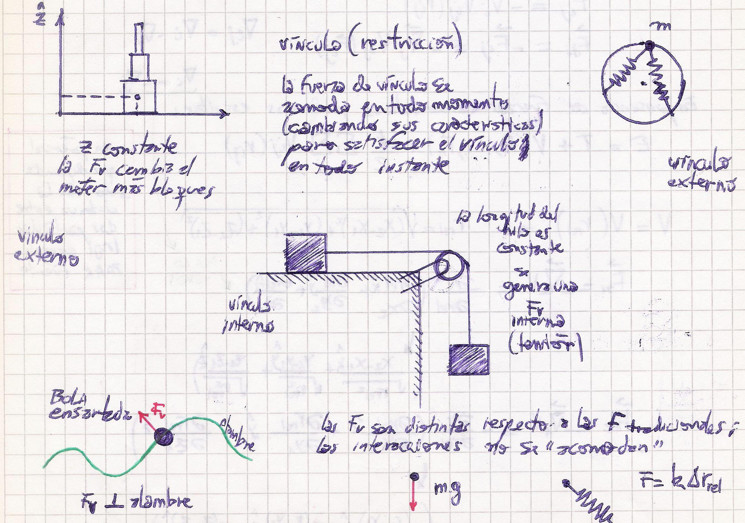
\includegraphics[width=0.85\textwidth]{images/fig_mc_vinculos_varios.jpg}	
	\caption{.}
	\label{fig_mc_vinculos_varios}
\end{figure} 

Las fuerzas de vínculo están asociadas a ecuaciones de vínculo y dependen de ellas. Las ecuaciones, además, {\it 
dependizan} las coordenadas de un problema. Examinemos un problema sencillo con vínculos.

\begin{ejemplo}{\bfseries Problema con fuerza de vínculo }

\label{problema_fuerza_vinculo}
Considerese el problema esquematizado en la figura donde dos bloques se mueven en un campo gravitatorio.
\begin{figure}[!ht]
	\centering
	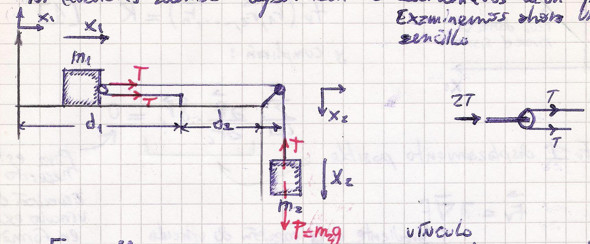
\includegraphics[width=0.5\textwidth]{images/fig_mc_problema_bloques.jpg}	
	\caption{.}
	\label{fig_mc_problema_bloques}
\end{figure} 
La segunda ley de Newton para cada bloque resultan en
\begin{align*}
	m_1 \ddot{x}_1 &= 2T \\
	m_2 \ddot{x}_2 &= m_2 g - T
\end{align*}
Pero la cuerda que une los dos cuerpos, suponiendo que se mantiene tensa en todo momento, vincula sus posiciones de 
manera que se debe cumplir 
\[
	2(d-x_1) + d_2 + x_2 = L
\]
Derivando dos veces esta relación se llega a
\[
	- 2\ddot{x}_1 + \ddot{x}_2 = 0,
\]
que al reemplazar en las ecuaciones de Newton permite, eliminando la tensión T, obtener
\[
	\ddot{x}_1 = \frac{2 m_2}{4m_2 + 1} \: g = \frac{1}{2 + 1/(2m_2)} \: g ,
\]
y
\[
	\ddot{x}_2 = \frac{4 m_2}{4m_2 + 1} \: g = \frac{1}{1 + 1/(4m_2)} \: g.
\]

Esto último nos dice que el bloque $m_2$ se moverá con aceleración $g$ en el límite de $m_2 \to \infty$ y el bloque
$m_1$ con aceleración $g/2$ bajo el mismo límite. 
\end{ejemplo}

El enfoque de Lagrange debiera permitir llegar a este mismo resultado por supuesto.

\notamargen{Si el vínculo es $f(\vb{x})=0$ entonces el trabajo virtual de las fuerzas es necesariamente nulo.}

% =================================================================================================
\section{Grados de libertad y vínculos}
% =================================================================================================

El número de grados de libertad es el número de coordenadas independientes para resolver el problema.

La interpretación lagrangiana encuentra las ecuaciones para las coordenadas independientes.
Dado un sistema con $N$ coordenadas y $k$ vínculos,
\[
	\# \text{ g. l. } = N - k \equiv \{ q_i \} \text{ coordenadas generalizadas}
\]

Consideremos el caso de una bola {\it ensartada} en un aro plano,

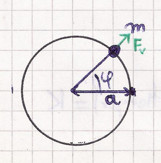
\includegraphics[scale=0.35]{images/fig_mc_bola_ensartada.jpg}

la cual puede moverse únicamente por el aro. Claramente la coordenada generalizada es $\varphi$, la cual
describe completamente el movimiento de la misma; el vínculo es $ r = a $ y el trabajo realizado por las
fuerzas de vínculo $W_{F_v} = 0 $ porque $F_v \perp \delta \varphi$. La fuerza de vínculo (en dirección radial)
es perpendicular al desplazamiento compatible con el vínculo.
En este caso el vínculo expresa las coordenadas del espacio real.

Las fuerzas de vínculo $\vb{F}^v$ se {\it acomodan} en todo momento para satisfacer las ligaduras.
Entonces las $\vb{F}^v$ son perpendiculares a los desplazamientos compatibles con los vínculos de
manera que 
\[
	W_{F^v} = 0,
\]
es decir que el trabajo virtual de las fuerzas de vínculo es nulo. Este trabajo puede no ser nulo si el tiempo 
varía (si no se considera un desplazamiento virtual).

\begin{figure}[hbt]
	\begin{center}
	\includegraphics[width=0.3\textwidth]{images/fig_mc_vinculos1.pdf}	 
	\includegraphics[width=0.3\textwidth]{images/fig_mc_vinculos2.pdf}
	\end{center}
	\caption{}
\end{figure} 

\notamargen{Un sistema 3D con dos vínculos resulta en un movimiento 1D; el sistema puede pensarse que se mueve sobre
un {\it alambre}.}

Para el caso de los bloques (o masas deslizantes), al tener dos coordenadas, el sistema se mueve en una recta del espacio 
de coordenadas.
La fuerza de vínculo es perpendicular al desplazamiento posible.
El vínculo expresa aquí las coordenadas donde se mueven las masas y el perpendicular al desplazamiento virtual pero no al
desplazamiento real.
\[
	\vb{F}_v = (2\vb{T}-\vb{T})
\]
\[
	V_{vy} = - \frac 1 2 F_{vx} (F_{vx},-\frac 1 2 F_{vx})
\]
El trabajo virtual de las fuerzas de vínculo es nulo.

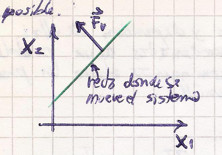
\includegraphics[scale=0.35]{images/fig_mc_problema_bloques_fases.jpg}
\notamargen{Entender este gráfico mejor!}

\begin{ejemplo}{\bf Aro acelerado en un plano}

Un aro que se mueve hacia la derecha con aceleración constante $\vb{a}$. 

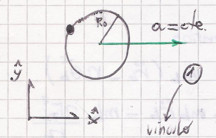
\includegraphics[scale=0.25]{images/fig_mc_aro_acelerado.jpg}

Tiene una ecuación de vínculo dada por 
\[
	(x-x_c)^2 + (y-y_c)^2 = R_0^2
\]
y donde 
\[
	x_c = x_0 + \frac 1 2 a t^2, \; y_c = y_0
\]
\end{ejemplo}

\subsection{Clasificación de los vínculos}

Los vínculos se clasifican en
\[
\textrm{holónomos} 
\begin{Bmatrix}
 f(r_i,t) = 0 \qquad \textrm{reónomos} \\
\; f(r_i) = 0 \qquad \textrm{esclerónomos} \;\\
\end{Bmatrix} 
\]
los cuales cumplen que  $W_{virtual}^{F^v}=0$, y
\[
\textrm{no holónomos} 
\begin{Bmatrix}
 f(r_i,t) \geq 0  \\
 f(r_i) \geq cte. \quad f(\dot{r}_i) = 0  \; \\
\end{Bmatrix}
\]
los cuales no cumplen, en general, que $\vb{F}^v$ perpendicular al desplazamiento posible.
\begin{figure}[hbt]
	\begin{center}
	\includegraphics[width=0.3\textwidth]{images/fig_mc_vinculos3.pdf}	
	\end{center}
	\caption{}
\end{figure} 
donde un desplazamiento virtual es un desplazamiento a $t_0$ fijo compatible con los vínculos,
mientras que un desplazamiento real es un desplazamiento en $\delta t$ durante el cual varían
fuerzas y ligaduras.

A tiempo fijo el desplazamiento es en $\hat{r} \perp \vb{F}^v$.
\[
	f(x_i,t) = cte. \Longrightarrow \sum_i^N \dpar{f}{x_i} \delta x_i + \dpar{f}{t} \delta t = 0 
\]
o bien
\[
	\nabla f \cdot \vb{\delta r} = 0
\]

Si las fuerzas de vínculo se pueden escribir como 
\[
	f_v(\vb{x}_1, \vb{x}_2, ..., \vb{x}_N ) = K,
\]
donde $K$ es una constante, luego (derivando implícitamente la ecuación) cumplirán
\[
	\sum_{i=1}^N \: \dpar{f_v}{\vb{x}_i}\:\delta{\vb{x}_i} = 0
\]
Entonces la fuerza de vínculo es proporcional al gradiente de la ecuación de vínculo,
\[
	\vb{F}_v = \lambda \nabla f
\]

En un caso 3D tendríamos
\[
	\dpar{f}{x}\delta x + \dpar{f}{y}\delta y + \dpar{f}{z}\delta z = 0
\]

Los vínculos que dependen de la velocidad o aquellos dados en términos de desigualdades (no de ecuaciones) no cumplen,
en general, que el trabajo de las fuerzas de vínculo sea perpendicular al desplazamiento.

La dependencia de las fuerzas de vínculo puede depender del tiempo. Supongamos ahora un problema parecido al anterior; 
una bola engarzada en una varilla que rota con velocidad angular constante $\omega$.

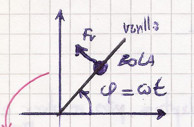
\includegraphics[scale=0.4]{images/fig_mc_bola_varilla_rotante.jpg}

La bola se mueve sobre la varilla; la coordenada angular $\varphi$ forma parte de la ecuación de vínculo
\[
	\varphi - \omega t = 0
\]
En un dado instante de tiempo fijo el único desplazamiento posible, que es en $\hat{r}$, es perpendicular a la fuerza 
de vínculo. No hay trabajo a tiempo fijo.
En estos casos la ecuación de vínculo será
\[
	f_v(\vb{x}_1, \vb{x}_2, ..., \vb{x}_N, t ) = K,
\]
pero como a tiempo fijo es $\Delta t=0$, se tiene 
\[
	\sum_{i=1}^N \: \dpar{f_v}{\vb{x}_i}\:\delta{\vb{x}_i} = 0
\]
donde no aparece al tiempo $t$.
Esto es un {\it desplazamiento virtual}; un desplazamiento a tiempo fijo compatible con los vínculos.

% =================================================================================================
\section{Velocidad y aceleración en coordenadas cilíndricas y esféricas}
% =================================================================================================

En la resolución de los problemas dinámicos que surgen de las ecuaciones de Newton la igualdad vectorial involucrada debe,
en general, escribirse en algún sistema de coordenadas apropiado. 
Esto implica para la aceleración la doble derivada con respecto al tiempo del vector de posición $ \vb{x}(t) $ en las
coordenadas en las cuales se halle escrito. 

Obviando el sistema cartesiano rectangular usual $(x,y,z)$, los dos sistemas de coordenadas más sencillos son el de
coordenadas cilíndricas $(r,\varphi,z)$ y el de coordenadas esféricas $(r,\theta,\varphi)$. Los problemas más sencillos
de la dinámica implican geometrías donde estos sistemas son apropiados. Asimismo, muchas geometrías más complejas pueden
quizás en primera aproximación modelarse con estas coordenadas.

Así, por ejemplo, un vector genérico en términos de la base de versores cilíndricos $(\hat{r},\hat{\varphi},\hat{z})$ será
\[
	\vb{V}(t) = r \hat{r} + \varphi \hat{\varphi} + z \hat{z},
\]
de manera que su derivada con respecto al tiempo implica la derivación de cada coordenada y cada versor.

La gran ventaja de las coordenadas cartesianas es que los versores $ \hat{ x }, \hat{ y }, \hat{ z }$ tienen su orientación
constante para cualquier punto del espacio, razón por la cual no varían con el tiempo. Entonces, en general, resulta 
conveniente evaluar las derivadas de los versores que sí varían con el tiempo (como por ejemplo $\hat{r}$) en términos de
su descomposición en cartesianas, puesto que sólo hay que derivar el coeficiente que lo acompaña.

Para coordenadas cartesianas, las fórmulas de velocidad y aceleración son triviales. A partir del vector de posición
\[
	\vb{x}(t) = x \hat{x} + y \hat{y}  + z\hat{z},
\]
se tienen 
\[
	\vb{v}(t) \equiv \dtot{\vb{x}}{t}(t) = \dot{\vb{x}}(t) = \dot{x} \hat{x} + \dot{y} \hat{y}  + \dot{z}\hat{z},
\]
\[
	\vb{a}(t) \equiv \dtot[2]{\vb{x}}{t}(t) = \ddot{\vb{x}}(t) = \ddot{x} \hat{x} + \ddot{y} \hat{y}  + \ddot{z} \hat{z},
\]
donde con el objeto de no sobrecargar la notación no se ha explicitado la dependencia temporal en las coordenadas.

A continuación se deducen las fórmulas de velocidad y aceleración para las coordenadas cilíndricas y esféricas a partir de
un vector de posición $ \vb{x}(t) $ del origen\footnote{Un vector del origen tiene su base anclada en el origen del sistema
de coordenadas lo que causa que no tenga componentes angulares en los sistemas cilíndrico y esférico. Esta simplificación
es importante y en realidad si no fuera aplicable la utilización de estos sistemas tal vez pierda su razón de ser.}.


\subsection{Coordenadas cilíndricas}

% La gran ventaja de las coordenadas cartesianas es que los versores $ \hat{i}, \hat{j}, \hat{k}$ no varían con el tiempo,
% entonces
% \[
% 	\vb{r}(t) = x \hat{i} + y \hat{j}
% \]
% lleva a que 
% \[
% 	\vb{v} = \dtot{\vb{r}}{t} = \dot{x}\hat{i} + \dot{y}\hat{j}
% \]
Un vector de posición del origen es 
\[
	\vb{x}(t) = r \:\hat{r} + z \:\hat{z},
\]
y la derivada temporal se hace con la regla de Leibniz en el caso del primer término de la derecha, 
\[
	\dtot{\vb{x}}{t} = \dtot{r}{t} \:\hat{r} + r \:\dtot{\hat{r}}{t} + \dtot{z}{t} \hat{z}
\]
y para evaluar la derivada temporal del versor consideramos la descomposición 
\[
	\hat{r} = \cos \varphi \:\hat{x} + \sin \varphi \:\hat{y}
\]
\notamargen{ 
% \begin{figure}[h]
% 	\begin{center}
	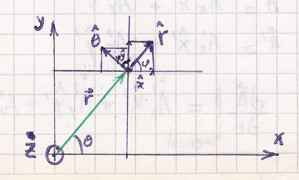
\includegraphics[scale=0.35]{images/fig_mc_polares_decomp.jpg}	
% 	\end{center}
% 	\caption{}
% \end{figure}
}
\[
	\hat{\varphi} = -\sin \varphi  \:\hat{x} + \cos  \varphi \:\hat{y}
\]
que lleva a 
\[
	\dtot{\hat{r}}{t} = - \sin \varphi \: \dot{ \varphi } \:\hat{x} + \cos \varphi \: \dot{ \varphi } \:\hat{y} =
	\dot{\vp} \: \hat{\vp}
\]
y entonces 
\[
	\dtot{\vb{x}}{t} = \dot{r} \:\hat{r } + r \:\dot{\vp} \: \hat{\vp} + \dot{z} \:\hat{z}.
\]

\notamargen{
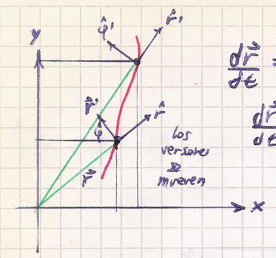
\includegraphics[scale=0.4]{images/fig_mc_polares_arbitrario.jpg}
}
% que se puede escribir como 
% \[
% 	\dtot{\vb{r}}{t} = \dot{r} \: \hat{r } + r \dot{\vp} \: \hat{\vp} = \dot{\vb{r}}
% \]
% y extraemos de conclusión que 
% \[
% 	\dtot{\hat{r}}{t} = \dot{\vp} \: \hat{\vp}
% \]

Para la aceleración hay que derivar la velocidad con respecto al tiempo
\[
	\ddot{\vb{x}} = \dtot{}{t} ( \dot{r} \: \hat{r} + r\dot{\vp} \: \hat{\vp} + \dot{z} \:\hat{z} ) 
\]
\[
	\ddot{\vb{x}} = \ddot{r} \:\hat{r} + \dot{r} \: \dtot{\hat{r}}{t} + \dot{r} \: \dot{\vp} \: \hat{\vp}
	+ r \left( \ddot{\vp} \: \phiver + \dot{\vp} \: \dtot{\hat{\vp}}{t} \right) + \ddot{z} \:\hat{z}
\]
y utilizando 
\[
	\dtot{\hat{\vp}}{t} = - \dot{ \vp } ( \cos \vp \:\hat{x} + \sin  \vp \:\hat{y} ) = - \dot{\vp} \: \hat{r}
\]
finalmente se arriba a
\[
	\ddot{\vb{x}} = ( \ddot{r} - r\dot{\vp}^2 ) \rver + ( r\ddot{\vp} + 2 \dot{r} \dot{\vp} ) \phiver + \ddot{z} \:\hat{z}.
\]

Para problemas de dos dimensiones suele utilizarse un sistema coordenado, conocido como coordenadas polares, que es el 
de cilíndricas con $ z \equiv 0 $. Las expresiones de velocidad y aceleración polares correspondientes serán las 
obtenidas en esta sección luego de {\it borrar} la coordenada $z$.

\subsection{Coordenadas esféricas}

Para el sistema esférico la deducción de la equivalencia cartesiana de los versores es un poco más trabajosa que en el 
sistema cilíndrico (donde en realidad estos versores viven en un plano $z$ cte.) y el álgebra implicado es algo 
engorroso. La expresión de los versores es
\[
	\rver = \cos\vp \sin\theta\xver + \sin\vp\sin\theta\yver + \cos\theta\zver,
\]
\[
	\phiver = -\sin\vp \xver + \cos\vp \yver,
\]
\[
	\thetaver = \cos\theta \cos\vp \xver + \cos\theta\sin\vp\yver - \sin\theta\zver.
\]
\notamargen{Dado que este es un curso básico pero que se jacata de visual, tendriamos que poner ilustraciones del 
carajo de los vectores en esféricas y cilíndricas para que quede intuitivo sus dificultades cuando el problema en
cuestión no tiene las simetrías explícitas de estos sistemas.}

Un vector de posición es simplemente
\[
	\vb{x} = r \rver
\]
aunque en el $\rver$ está {\it escondida} la dependencia angular. Consignaremos a continuación solamente las 
expresiones finales para la velocidad y aceleración, que son respectivamente
\[
	\vb{v} = \dot{\vb{x}} = \dot{r} \rver + r\dot{\theta}\thetaver + r\dot{\vp}\sin\theta\phiver
\]
\begin{multline*} % \vb no se da cuenta que multline ES modo matemático (por ello el .\ inicial)
	\!\: \vb{a} = \ddot{\vb{x}} = ( \ddot{r} - r\dot{\theta}^2 - r\dot{\vp}^2 \sin^2 \theta )\rver +
	( r\ddot{\theta} + 2\dot{r}\dot{\theta} - r\dot{\vp}^2 \sin \theta \cos\theta )\thetaver \: + \\
	( r \ddot{\vp}\sin\theta + 2 \: \dot{r} \: \dot{\vp} \sin\theta + 2 \: r \:\dot{\theta} \:\dot{\vp} \cos\theta )\phiver 
\end{multline*}
	

% =================================================================================================
\section{Transformación entre sistemas en rotación}
% =================================================================================================

Otro tipo de transformación común entre sistemas de coordenadas (en el plano) que comparten origen es la rotación.

Suponiendo un sistema de coordenadas $(x,y)$ fijo (que llamaremos ``inercial'') de origen $O$ y otro de coordenadas 
$(x',y')$, que está rotando en torno a ese origen (sistema ``móvil''), interesa ver qué consecuencias tiene sobre la 
velocidad y aceleración de un vector de posición \vb{A}, el hecho de determinarlas desde uno u otro sistema. Si bien 
hablamos de un sistema {\it fijo}, en realidad ambos se hallan en rotación entre sí. 

Como se ve en la FIGURA XXX 
\notamargen{
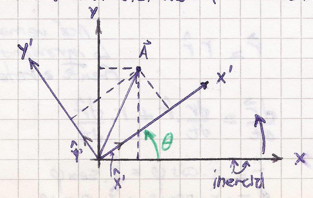
\includegraphics[scale=0.4]{images/fig_mc_sist_rotantes.jpg}
}
la posición instantánea entre sistemas está determinada por el ángulo $\theta(t)$ y, dado que ambos sistemas comparten 
el origen, los mismos son coincidentes en $\theta = 0$. 
% Como el sistema en rotación varía la posición de sus ejes con el tiempo, sus versores asociados $(\xver', \yver')$ 
% también variarán con el tiempo (pese a que son cartesianos).

Dado que los sistemas no se hallan entre sí a velocidad constante\footnote{Aún en el caso de $ \theta(t) = cte.$ la 
velocidad no es constante como vector puesto que cambia de dirección todo el tiempo.} es patente que las ecuaciones de 
Newton se verán modificadas.
Para un vector \vb{A} constante con respecto al sistema inercial, cualitativamente esperaríamos observarlo desde el 
sistema móvil en alguna suerte de movimiento dado por el efecto dinámico de la rotación\footnote{Si estoy montado en el 
caballo de madera de una calesita veré a mi abuela, que me espera inmóvil a un lado, como dotada de movimiento.}. Veamos 
qué surge de la cuenta algebraica.

El mismo vector de acuerdo a los dos sistemas de coordenadas en el plano, es
\[
	\vb{A}(t) = A_x\xver + A_y\yver         \qquad\qquad               \vb{A}'(t) = A_x'\xver' + A_y'\yver'
\]
donde las coordenadas primadas refieren al sistema móvil. Nótese que los versores asociados en ambos casos $(\xver, 
\yver)$ y $(\xver', \yver')$ son constantes, esto es, no dependen del tiempo. Que ambos sistemas se hallen en rotación 
entre sí no es intrínseco de alguno de ellos.
Un observador del sistema primado ve a sus ejes fijos mientras que en las medidas que realiza sobre \vb{A} verá una 
dinámica particular. 

Si consideramos la variación temporal de \vb{A}' pero como es vista desde el sistema inercial resulta 
\[
	\left. \dtot{\vb{A}}{t} \right|_\text{inercial} = 
	\dot{A_x'} \xver' + A_x'\dot{\xver'} + \dot{A_y'}\yver' + A_y' \dot{\yver'},
\]
porque para un observador en el sistema inercial se mueven las componentes del vector y los versores.

\notamargen{Esta notación es oscura, habría que ver una mejor manera de explicar esto.}

La variación temporal de los versores la conocemos porque es la misma situación geométrica que la encontrada para el 
caso de los versores cilíndricos $(\rver,\phiver)$. Podemos hallar la equivalencia
\[
	\dtot{\hat{x}'}{t} = \dot{\theta} \yver'         \qquad \qquad          \dtot{\hat{y}'}{t} = -\dot{\theta} \xver'.
\]

Desde el sistema móvil los versores son por supuesto constantes (el sistema móvil no es consciente de su movimiento) de 
modo que 
\[
	\left. \dtot{\vb{A}}{t} \right|_\text{móvil} = \dot{A_x'}\xver' + \dot{A_y'}\yver'
\]
y entonces
\[
	\left. \dtot{\vb{A}}{t} \right|_\text{fijo} = \left. \dtot{\vb{A}}{t} \right|_\text{móvil}
	+ A_x' \dot{\theta}\yver' - A_y'\dot{\theta}\xver'.
\]
% donde 
% \[
% 	\left. \dtot{\vb{A}'}{t} \right|_\text{móvil} \equiv \sum_i \dtot{A_i'}{t} \: \hat{e_i}'
% \]
% \[
% 	\left. \dtot{\vb{A}}{t} \right|_\text{móvil} = \dot{A_x'}\xver' + \dot{A_y'}\yver'
% \]

Si definimos
\[
	\vb{\omega} = \dot{\theta} \zver,
\]
entonces resulta que
\[
	\vb{\omega}\times\vb{A}' = \dot{\theta} \zver \times ({A_x'}\xver' + {A_y'}\yver') =
	A_x' \dot{\theta}\yver' - A_y'\dot{\theta}\xver'.
\]

Volviendo a la derivada de \vb{A} tenemos
\[
	\left. \dtot{\vb{A}}{t} \right|_\text{fijo} = \left. \dtot{\vb{A}}{t} \right|_\text{móvil}
	+ \vb{\omega} \times \vb{A}'
\]
que nos da la variación temporal de un vector \vb{A} visto desde un sistema fijo en términos de lo que se mediría
en un sistema (móvil) que está en rotación respecto al primero.

Si ahora la especializamos para un vector de posición \vb{x}, obtenemos la velocidad  
\[
	\left. \vb{v} \right|_\text{fijo} = \left. \vb{v} \right|_\text{móvil} + \vb{\omega} \times \vb{x}',
\]
donde 
\[
	\left. \vb{v} \right|_\text{móvil} = \dot{x}' \xver' + \dot{y}' \yver' 
\]

Asimismo, la aceleración se obtiene aplicando la relación al vector $\vb{v} \equiv d\vb{x}/dt$, de manera que 
tendremos
\[
	\left. \vb{a} \right|_\text{fijo} = \left. \dtot{\vb{v}}{t} \right|_\text{fijo} = \left. \dtot{\vb{v}}{t} \right|_\text{móvil} +
	\vb{\omega} \times \vb{v}'
\]
\[
	\left. \vb{a} \right|_\text{fijo} = 
	\dtot{}{t}\left[ \left. \dtot{\vb{x}}{t} \right|_\text{móvil} + \vb{\omega}\times\vb{x}' \right] +
	\vb{\omega} \times \left[ \left. \vb{v} \right|_\text{móvil} +	\vb{\omega}\times\vb{x}' \right]
\]

Ahora procedemos a trabajar las expresiones dentro del primer corchete, empezando por la derivada temporal de la velocidad
en el sistema móvil,
\[
	\left. \vb{a} \right|_\text{móvil} \equiv  
	\dtot{}{t}\left.( \dot{x}' \xver' + \dot{y}' \yver' )\right|_\text{móvil} = \ddot{x}' \xver' + \ddot{y}' \yver'
\]
y continuando con el término 
\[
	\left.\vb{\omega}\times\vb{x}'\right|_\text{móvil} = \omega x' \yver' - \omega y' \xver' ,
\]
cuya derivada es
\[
	\dtot{}{t}\left.\vb{\omega}\times\vb{x}\right|_\text{móvil} = 
	-( \dot{\omega} y' + \omega \dot{y}' )\xver' + ( \dot{\omega} x' + \omega \dot{x}' )\yver' =
	\left. \vb{\omega} \times\vb{v}'\right|_\text{móvil} + \left.\dot{\vb{\omega}} \times\vb{x}'\right|_\text{móvil}
\]

Juntando todo resulta
\[
	\left. \vb{a}\right|_\text{fijo} = \left. \vb{a}\right|_\text{móvil} 
	+ \left.\dot{\vb{\omega}} \times\vb{x}'\right|_\text{móvil} + 2 \:\vb{\omega}\times\vb{v'} + \vb{\omega}
	\times (\vb{\omega} \times \vb{x}')
\]
donde el tercero es la aceleración de Coriolis y el cuarto la aceleración centrípeta.

Las leyes de Newton observadas desde el sistema fijo serán 
% Llamando $ \alpha = \dot{\omega} = \dtot{\omega}{t}$ resulta 
\[
	\vb{F} = m\vb{a} = m \left. \vb{a}\right|_\text{móvil} + m \: \dot{ \vb{\omega} } \times \vb{r} + 4 \: m \: 
	\vb{\omega}\times\vb{v'} + m \: [  \vb{\omega} \times (\vb{\omega}\times\vb{r} )]
\]
que se pueden reacomodar como  
\[
	m \left. \vb{a}\right|_\text{fijo} = 
	\vb{F} - m \left. \vb{a}\right|_\text{móvil} - m \: \dot{\vb{\omega}} \times \vb{r} - 4 \: m \: \vb{\omega}\times\vb{v'} -
	m \: [\vb{\omega} \times(\vb{\omega}\times\vb{r})]
\]
donde ahora en el RHS tenemos la fuerza $\vb{F}$ que es la única que produce par de acción y reacción, y los términos de 
fuerza lineal, de Coriolis y centrífuga.

Si $\vb{\omega} = cte.$ entonces la fuerza lineal es nula.

\notamargen{Está un poco inconsistente la notación utilizada, con lo de móvil y la prima. La carpeta tiene muchos
typos. El 'Problema' de la hoja 5R no lo entiendo; en realidad parece estar vinculado a sólidos. Habría que decidir si 
ponerlo o no. En caso negativo, ¿qué otro se puede ubicar?}

\begin{notasfinales}

\label{nota_suma_ineqj}
\item{ \bf Sumatoria de torques}
Una manera de convencerse de que esta escritura es posible es hacer un diagrama de los diferentes términos que
aparecen en esta doble sumatoria. Es fácil de ver que con el añadido del término $\vb{x}_j \times \vb{F}_{ji} $ se está 
haciendo un doble conteo que justifica el $1/2$ que aparece luego.

Una demostración más matemática puede lograrse escribiendo la sumatoria $ j\neq i $ sin esta restricción, lo cual se 
puede hacer así:
\[
	\Sum{i=1}{N} \Sum{j\neq i}{N}  \vb{x}_i \times \vb{F}_{ij} = 
	\Sum{i=1}{N} \Sum{j=1}{N}  \vb{x}_i \times \vb{F}_{ij} ( 1 - \delta_{ij} )
\]
siendo $ \delta_{ij} $ la delta de Kronecker. Es claro que podemos hacer un cambio de etiquetas en las sumatorias 
puesto que los índices sumados son {\it mudos}, i.e.
\[
	\Sum{i=1}{N} \Sum{j=1}{N}  \vb{x}_i \times \vb{F}_{ij} ( 1 - \delta_{ij} ) = 
	\Sum{j=1}{N} \Sum{i=1}{N}  \vb{x}_j \times \vb{F}_{ji} ( 1 - \delta_{ij} )
\]
y dado que el orden de las sumatorias es irrelevante llegamos a
\[
	\Sum{i=1}{N} \Sum{j\neq i}{N}  \vb{x}_i \times \vb{F}_{ij} = \frac{1}{2}
	\Sum{i=1}{N} \Sum{j=1}{N} \left[ \vb{x}_i \times \vb{F}_{ij} ( 1 - \delta_{ij} ) +
	\vb{x}_j \times \vb{F}_{ji} ( 1 - \delta_{ij} )
	\right] 
\]

Regresando ahora a las sumatoria restringida obtenemos 
\[
	\Sum{i=1}{N} \Sum{j\neq i}{N}  \vb{x}_i \times \vb{F}_{ij} = \frac{1}{2}
	\Sum{i=1}{N} \Sum{j \neq i }{N} \left[ \vb{x}_i \times \vb{F}_{ij} + \vb{x}_j \times \vb{F}_{ji} \right] 
\]
que es el resultado buscado.


\end{notasfinales}


% ============================================================================

% \bibliographystyle{CBFT-apa-good} % (uses file "apa-good.bst")
% \bibliography{CBFT.Referencias} % La base de datos bibliográfica


\end{document}
